
\chapter{GCSE Revision - Algebraic Proof and Algebra in Context}

\begin{enumerate}
  \item Use algebra to prove that the sum of three consecutive whole numbers is always divisible by $3$.\strch
  \item Prove that $(2n + 3)^2 - (2n - 3)^2$ is a multiple of $8$ for all positive integer values of $n$.\strch
  \item The diagram shows a trapezium.
  \begin{figure}[H]
    \centering
    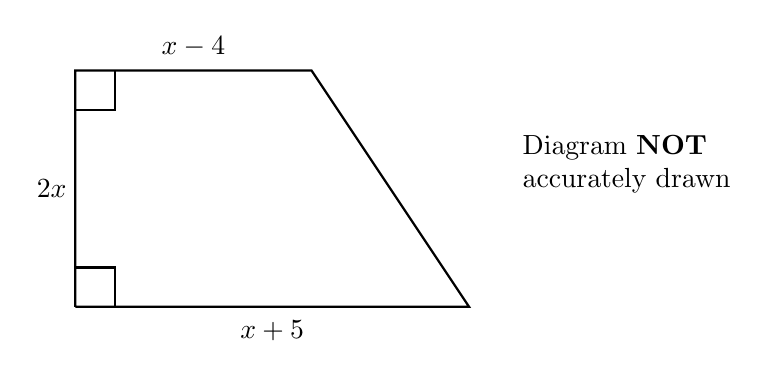
\begin{tikzpicture}
      \draw[thick] (0, 0) -- (5, 0) -- (3, 3) -- (0, 3) -- (0, 0);
      \node at (2.5, -0.3) {$x + 5$};
      \node at (-0.3, 1.5) {$2x$};
      \node at (1.5, 3.3) {$x - 4$};

      \draw[thick] (0, 0.5) -- (0.5, 0.5) -- (0.5, 0);
      \draw[thick] (0, 2.5) -- (0.5, 2.5) -- (0.5, 3);

      \node[label={[align=left]Diagram \textbf{NOT}\\accurately drawn}] at (7, 1.2) {};
    \end{tikzpicture}
  \end{figure}
  %
  All the measurements are in centimetres.\\
  The area of the trapezium is $351 cm^2$.
  \newpage
  \begin{enumerate}
    \item Show that $2x^2 + x - 351 = 0$.\mrk{2}\strch
    \item Work out the value of $x$.\mrk{3}\strch
  \end{enumerate}
  \item Here are two triangles $\vb{T_1}$ and $\vb{T_2}$.
  %
  \begin{figure}[H]
    \centering
    \begin{tikzpicture}[scale=0.8]
      \coordinate (A) at (-1, 0);
      \coordinate (B) at (-7, 0);
      \coordinate (C) at (-2, 4);

      \coordinate (X) at (0.5, 0);
      \coordinate (Y) at (3.5, 0);
      \coordinate (Z) at (3.5, 4.5);

      \coordinate (a1) at (-3.5, -0.2);
      \coordinate (a2) at (-4.7, 2.2);

      \coordinate (x1) at (2, -0.2);
      \coordinate (x2) at (4.2, 2.25);

      \coordinate (text) at (7.5, 2);

      \draw[thick] (A) -- (B) -- (C) -- (A);
      \draw[thick] (X) -- (Y) -- (Z) -- (X);

      \node at (-3.33, 1.33) {$\vb{T_1}$};
      \node at (2.5, 1.5) {$\vb{T_2}$};

      \begin{scope}
        \path[clip] (A) -- (B) -- (C);
        \draw (B) circle (15mm);
        \node at ($(B)+(20:10mm)$) {$\ang{30}$};
      \end{scope}

      \node at (a1) {$x$};
      \node at (a2) {$x$};

      \node at (x1) {$x - 2$};
      \node at (x2) {$x + 1$};

      \node[label={[align=left]Diagram \textbf{NOT} \\ accurately drawn}] at (text) {};
    \end{tikzpicture}
  \end{figure}
  %
  The lengths of the sides are in centimetres.\\
  The area of triangle $\vb{T_1}$ is equal to the area of triangle $\vb{T_2}$.\\
  Work out the value of $x$, giving your answer in the form $a + \sqrt{b}$ where $a$ and $b$ are integers.\strch
  \item Prove algebraically that the difference between the squares of any two consecutive integers is equal to the sum of these two integers.\strch
  \newpage
  \item \mbox{}
  \begin{figure}[H]
    \centering
    \begin{tikzpicture}[scale=1.5]
      \coordinate (B) at (0, 0);
      \coordinate (A) at (0, 4);
      \coordinate (C) at (4, 0);
      \coordinate (D) at (4, 4);

      \coordinate (M) at (4, 2);
      \coordinate (N) at (2.5, 4);

      \coordinate (varr1) at (0-0.1, 4);
      \coordinate (varr2) at (0-0.1, 0);

      \coordinate (harr1) at (4, 4+0.1);
      \coordinate (harr2) at (2.5, 4+0.1);

      \coordinate (t1) at (0, 2);
      \coordinate (t2) at (3.25, 4);

      \draw (A) -- (B) -- (C) -- (D) -- (A);

      \node at (A) [above left = 0.1mm of A] {$A$};
      \node at (B) [below left = 0.1mm of B] {$B$};
      \node at (C) [below right = 0.11mm of C] {$C$};
      \node at (D) [above right = 0.1mm of D] {$D$};

      \tkzMarkRightAngle (A,B,C);
      \tkzMarkRightAngle (B,C,D);
      \tkzMarkRightAngle (D,A,B);
      \tkzMarkRightAngle (A,D,C);

      \draw[color=black, fill=gray, opacity=0.6] (B) -- (M) -- (N) -- (B);
      \tkzMarkRightAngle (B,M,N);

      \node at (M) [right = 0.1mm of M] {$M$};
      \node at (N) [above left = 0.1mm of N] {$N$};

      \draw[>=triangle 45, <->] (varr1) -- (varr2);
      \draw[>=triangle 45, <->] (harr1) -- (harr2);

      \node at (t1) [left = 1.2mm of t1] {$4x$};
      \node at (t2) [above = 1.2mm of t2] {$x$};

      \node[label={[align=left]Diagram \textbf{NOT} \\ accurately drawn}] at (M) [right = 3cm of M] {};
    \end{tikzpicture}
  \end{figure}
  %
  $ABCD$ is a square with a side length of $4x$.\\
  $M$ is the midpoint of $DC$.\\
  $N$ is the point on $AD$ where $ND = x$.\par
  $BMN$ is a right-angled triangle.\par
  Find an expression, in terms of $x$, for the area of triangle $BMN$.\\
  Give your expression in its simplest form.\strch
  \newpage
  \item \mbox{}
  \begin{figure}[H]
    \centering
    \begin{tikzpicture}
      \coordinate (P) at (0, 0);
      \coordinate (Q) at (4, 0);
      \coordinate (R) at (5, 3.5);

      \draw (P) -- (Q) -- (R) -- (P);

      \node at (P) [left = 1mm of P] {$P$};
      \node at (R) [above = 1mm of R] {$R$};
      \node at (Q) [right = 1mm of Q] {$Q$};

      \begin{scope}
        \path[clip] (R) -- (P) -- (Q);
        \draw (P) circle (15mm);
        \node at ($(P)+(20:10mm)$) {$\ang{30}$};
      \end{scope}

      \node at ($(P)+(45:3cm)$) {$2x\ cm$};
      \node at ($(P)+(-5.5:2.5cm)$) {$x\ cm$};

      \node[label={[align=left]Diagram \textbf{NOT} \\ accurately drawn}] at (R) [below right = 3cm of R] {};
    \end{tikzpicture}
  \end{figure}
  %
  $PQ = x\ cm$\\
  $PR = 2x\ cm$\\
  Angle $QPR = \ang{30}$\par
  The area of triangle $PQR = A\ cm^2$\\
  Show that $x = \sqrt{2A}$.\strch
  \item \mbox{}
  \begin{figure}[H]
    \centering
    \begin{tikzpicture}[scale=1.2]
      \coordinate (P) at (0, 0);
      \coordinate (Q) at (6, 0);
      \coordinate (R) at (0, 3);

      \draw (P) -- (Q) -- (R) -- (P);

      \tkzMarkRightAngle (R,P,Q);

      \node at ($(P)+(32:3.7cm)$) {$3x + 1$};
      \node at ($(P)+(-5.5:2.5cm)$) {$3x$};
      \node at ($(P)+(110:1.5cm)$) {$x-1$};

      \node[label={[align=left]Diagram \textbf{NOT} \\ accurately drawn}] at (Q) [above right = 3cm of Q] {};
    \end{tikzpicture}
  \end{figure}
  %
  In the diagram, all the measurements are in metres.\par
  The perimeter of the triangle is $56$ m.\\
  The area of the triangle is $A$ $\text{m}^2$.\par
  Work out the value of $A$.\strch
  \newpage
  \item \mbox{}
  \begin{figure}[H]
    \centering
    \begin{tikzpicture}[scale=0.8]
      \draw (0,0) circle (2cm and 0.5cm);
      \draw(2,0) -- (0,4) -- (-2,0);
      \draw (2,0) -- node[below] {$x$} (0,0) -- node[left] {$h$} (0,4) ;

      \draw (5,0) circle (2cm and 0.5cm);
      \draw (3,0) arc (180:0:2);

      \draw[>=triangle 45, <->] (5,0) -- node[below] {$x$} (7,0);

      \node[label={[align=left]Diagram \textbf{NOT} \\ accurately drawn}] at (9, 2) {};
    \end{tikzpicture}
  \end{figure}
  %
  The diagram shows a solid cone and a solid hemisphere.\\
  The cone has a base of radius $x$ cm and a height of $h$ cm.\\
  The hemisphere has a base of radius $x$ cm.\\
  The surface area of the cone is equal to the surface area of the hemisphere.\par
  Find an expression for $h$ in terms of $x$.\strch
  \item Umar thinks $(a + 1)^2 = a^2 + 1$ for all values of $a$.
  \begin{enumerate}
    \item Show that Umar is wrong.\mrk{2}\strch
    \item Here are two right-angled triangles.\\
    All the measurements are in centimetres
    \begin{figure}[H]
      \centering
      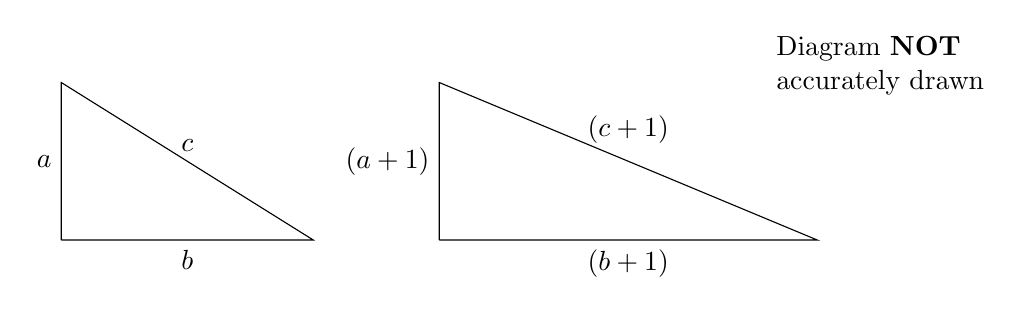
\begin{tikzpicture}[scale=0.8]
        \coordinate (A1) at (0, 0);
        \coordinate (B1) at (4, 0);
        \coordinate (C1) at (0, 2.5);

        \coordinate (A2) at (6, 0);
        \coordinate (B2) at (12, 0);
        \coordinate (C2) at (6, 2.5);

        \draw (A1) -- node[left] {$a$} (C1) -- node[above] {$c$} (B1) -- node[below] {$b$} (A1);
        \tkzMarkRightAngle (B1,A1,C1);

        \draw (A2) -- node[left] {$(a+1)$} (C2) -- node[above=1mm] {$(c+1)$} (B2) -- node[below] {$(b+1)$} (A2);
        \tkzMarkRightAngle (B2,A2,C2);

        \node[label={[align=left]Diagram \textbf{NOT} \\ accurately drawn}] at (13, 2) {};
      \end{tikzpicture}
    \end{figure}
    %
    Show that $2a + 2b + 1 = 2c$. $a,\ b$ and $c$ cannot all be integers.\mrk{3}\strch
    \newpage
    \item Explain why.\mrk{1}\strch
  \end{enumerate}
  \item The diagram below shows a large rectangle of length $(2x + 6)$ cm and width $x$ cm. A smaller rectangle of length $x$ cm and width $3$ cm is cut out and removed.
  %
  \begin{figure}[H]
    \centering
    \begin{tikzpicture}
      \coordinate (A1) at (0, 0);
      \coordinate (B1) at (5, 0);
      \coordinate (C1) at (5, 3);
      \coordinate (D1) at (0, 3);

      \coordinate (A2) at (3, 0);
      \coordinate (B2) at (3, 1.5);
      \coordinate (C2) at (5, 1.5);

      \coordinate (varr1) at (3, -0.2);
      \coordinate (varr2) at (5, -0.2);

      \coordinate (harr1) at (5.2, 0);
      \coordinate (harr2) at (5.2, 1.5);

      \draw (A1) -- (B1) -- (C1) -- node[above] {$2x + 6$} (D1) -- node[left] {$x$} (A1);
      \draw[color=black, fill=gray, opacity=0.6] (A2) -- (B2) -- (C2) -- (B1) -- (A2);

      \draw[>=triangle 45, <->] (varr1) -- node[below] {$x$} (varr2);
      \draw[>=triangle 45, <->] (harr1) -- node[right] {$3$} (harr2);
    
      \node[label={[align=left]Diagram \textbf{NOT} \\ accurately drawn}] at (8, 2) {};
    \end{tikzpicture}
  \end{figure}
  %
  The area of the shape that is left is $100$ $\text{cm}^2$
  \begin{enumerate}
    \item Show that $2x^2 + 3x - 100 = 0$.\mrk{3}\strch
    \item Calculate the length of the smaller rectangle. Give your answer correct to $3$ significant figures.\mrk{4}\strch
  \end{enumerate}
  \newpage
  \item \mbox{}
  \begin{figure}[H]
    \centering
    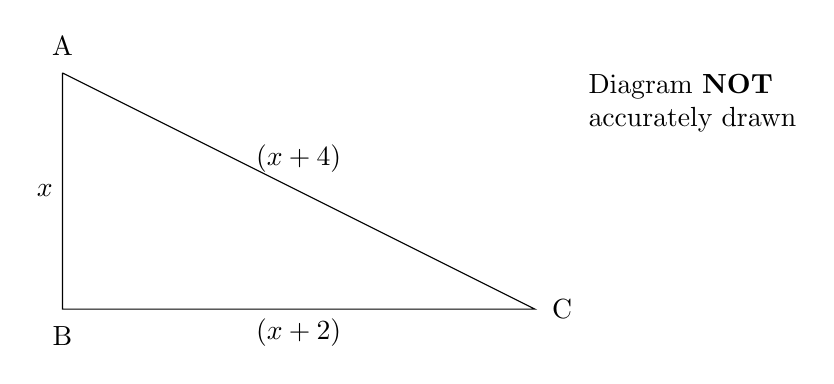
\begin{tikzpicture}
      \coordinate (B1) at (0, 0);
      \coordinate (A1) at (0, 3);
      \coordinate (C1) at (6, 0);

      \draw (A1) -- node[left] {$x$} (B1) -- node[below] {$(x+2)$} (C1) -- node[above=1.1mm] {$(x+4)$} (A1);
      \tkzMarkRightAngle (A1,B1,C1);

      \node[label=above:A, scale=0.75] (A1) at (A1) {};
      \node[label=below:B, scale=0.75] (B1) at (B1) {};
      \node[label=right:C, scale=0.75] (C1) at (C1) {};

      \node[label={[align=left]Diagram \textbf{NOT} \\ accurately drawn}] at (8, 2) {};
    \end{tikzpicture}
  \end{figure}
  %
  ABC is a right-angled triangle.\\
  All the measurements are in centimetres.\par
  $AB = x$\\
  $BC = (x + 2)$\\
  $AC = (x + 4)$
  \begin{enumerate}
    \item Show that $x^2 - 4x - 12 = 0$.\mrk{3}\strch
    \item \hfill\mrk{4}
    \begin{enumerate}
      \item Solve $x^2 - 4x - 12 = 0$\strch
      \item Hence, write down the length of $AC$.\strch
    \end{enumerate}
  \end{enumerate}
  \item Prove that the difference between the squares of two consecutive odd numbers is a multiple of $8$.\strch
  \newpage
  \item Prove that $n^2 + n + 1$ is always odd for all integers $n$.\strch
  \item Factorise $2t^2 + 5t + 2$. Hence explain why $2t^2 + 5t + 2$ can never be a prime number for any positive whole number value of $t$.\strch
\end{enumerate}